\documentclass[journal]{IEEEtran}
\usepackage[utf8]{inputenc}
\usepackage[T1]{fontenc}
\usepackage[spanish,es-tabla,es-nodecimaldot]{babel}
\usepackage{amsmath,amssymb,graphicx,booktabs,tikz,cite}
\usetikzlibrary{arrows.meta,positioning,fit,babel}
\graphicspath{{figs/}}
\renewcommand{\figurename}{Figura}
\renewcommand{\tablename}{Tabla}
\makeatletter
\renewcommand{\thetable}{\arabic{table}}
\def\fnum@table{\tablename~\thetable.}
\def\fnum@figure{\figurename~\thefigure}
\renewcommand{\abstractname}{Abstract}
\renewcommand{\IEEEkeywordsname}{Palabras clave}
\makeatother
\hyphenation{co-di-fi-ca-dor de-co-di-fi-ca-dor}

\begin{document}
\title{Esteganografía de audio por enmascaramiento con eco: codificador por convolución y decodificador por autocorrelación del cepstro}
\author{\IEEEauthorblockN{Noel Perez Caceres - }
\IEEEauthorblockA{Escuela de Ingeniería Electrónica, Instituto Tecnológico de Costa Rica\\
Procesamiento Digital de Señales, Maestría en Electrónica, 2026}}
\maketitle

\begin{abstract}
This paper presents a steganographic system for digital audio based on echo hiding. Metadata bits are embedded into 16-bit, 44.1~kHz stereo WAV files by convolving fixed-length windows with one of two linear time-invariant (LTI) systems that add an echo with a bit-dependent delay, combining the windows with overlap-and-add. The decoder computes the autocorrelation of the cepstrum in the spectral domain and compares its magnitude at both delays. To survive signal-dependent errors, the bit stream is protected with a Hamming(7,4) code and a cyclic redundancy check (CRC), repeated cyclically over the whole file, and the copies are soft-combined at the decoder. Experiments on three public-domain or Creative Commons tracks (classical, jazz and folk) show a window recovery rate above 96\% with the default parameters (echo amplitude 30\%, delays 1 and 2~ms), a throughput of 62.6~b/s, perceptual evaluation of speech quality (PESQ) between 2.7 and 4.0, and full metadata recovery from 30~s of audio. The recovery rate increases with echo amplitude and window length, at the expense of perceptual quality and throughput.
\end{abstract}

\begin{IEEEkeywords}
autocorrelación del cepstro, convolución, enmascaramiento con eco, esteganografía, solapamiento y suma
\end{IEEEkeywords}

\section{Introducción}
La esteganografía codifica un mensaje dentro de una señal portadora de modo que pase inadvertido, aprovechando las limitaciones perceptuales humanas. En audio se aplica a la protección contra piratería, a las restricciones geográficas de contenido y a la adición de metadatos. Entre las técnicas existentes están la codificación de bits, el espectro disperso, la codificación de fase y el enmascaramiento con eco \cite{kim,behal}. Esta última, propuesta por Gruhl y Bender \cite{gruhl}, es de especial interés porque cada componente interno es un sistema lineal e invariante en el tiempo (LTI, del inglés \textit{linear time-invariant}) y se analiza con herramientas como la convolución y el cepstro. Korzhik \cite{korzhik} estudia su variante con probabilidad de error nula.

Este trabajo implementa un codificador y un decodificador de enmascaramiento con eco. El prototipo se desarrolló en Python y la versión final en C++ para GNU/Linux. Las contribuciones son: (i) una elección de ventana justificada experimentalmente; (ii) un protocolo de metadatos con corrección de errores que se repite cíclicamente por el archivo; y (iii) una caracterización con calidad perceptual, tasa de recuperación y tasa de transferencia sobre tres géneros musicales.

El resto del documento se organiza así: la sección~II resume la teoría; la sección~III describe la solución; la sección~IV presenta y analiza los resultados; y la sección~V expone las conclusiones y el trabajo futuro.

\section{Marco teórico}
\subsection{Enmascaramiento con eco}
Cada bit $b\in\{0,1\}$ se codifica con el sistema
\begin{equation}
H_b(z)=1+a_b z^{-t_b},
\label{eq:hb}
\end{equation}
cuya respuesta al impulso $h_b(n)=\delta(n)+a_b\delta(n-t_b)$ tiene longitud $N=t_b+1$. Los retardos se dan en microsegundos $d_b$ y las amplitudes en porcentaje $p_b$ con respecto a la señal original, de modo que $t_b=\mathrm{round}(d_b\,10^{-6}f_s)$ y $a_b=p_b/100$, con $f_s=44\,100$~Hz. Al convolucionar una ventana de longitud $M$ con $h_b$ el resultado tiene $M+N-1$ muestras; el excedente de $N-1$ debe sumarse a la ventana siguiente (solapamiento y suma), de lo contrario aparecen componentes espectrales parásitas.

\subsection{Cepstro y su autocorrelación}
El cepstro de una señal es $c(n)=\mathcal{F}^{-1}\{\ln(\mathcal{F}\{x(n)\})\}$ y su autocorrelación se evalúa en el dominio espectral como
\begin{equation}
R_{cc}(n)=c(n)*c(n)=\mathcal{F}^{-1}\left\{\left(\ln|\mathcal{F}\{x(n)\}|\right)^{2}\right\}.
\label{eq:rcc}
\end{equation}
Un eco de retardo $t$ y amplitud $a$ introduce un rizado multiplicativo $|1+ae^{-j\omega t}|$ en el espectro; su logaritmo es aditivo y produce picos del cepstro en $t,2t,\dots$, que $R_{cc}$ destaca.

\section{Solución propuesta}
La Figura~\ref{fig:bloques} resume el sistema. Los parámetros por defecto son $d_0=1$~ms, $d_1=2$~ms ($t_0=44$ y $t_1=88$ muestras) y $a_0=a_1=0.3$.

\begin{figure}[t]
\centering
\begin{tikzpicture}[font=\scriptsize,>=Stealth,node distance=2.2mm,
 b/.style={draw,rounded corners=1pt,minimum height=6.5mm,minimum width=9mm,align=center,inner sep=1.5pt}]
\node[b] (x) {$x(n)$};
\node[b,right=of x] (w) {Enventa-\\nado};
\node[b,right=of w] (h) {$H_0$ o $H_1$\\(convol.)};
\node[b,right=of h] (o) {Solap. y\\suma};
\node[b,right=of o] (y) {$y(n)$};
\node[b,above=3mm of h] (m) {Bits:\\Hamming+CRC};
\draw[->] (x)--(w); \draw[->] (w)--(h); \draw[->] (h)--(o); \draw[->] (o)--(y); \draw[->] (m)--(h);
\node[b,below=7mm of x] (y2) {$y(n)$};
\node[b,right=of y2] (w2) {Enventa-\\nado};
\node[b,right=of w2] (r) {$R_{cc}$ (con y\\sin Hann)};
\node[b,right=of r] (c) {$z_0,z_1$ y\\suma de\\copias};
\node[b,right=of c] (d) {Hamming,\\CRC y\\metadatos};
\draw[->] (y2)--(w2); \draw[->] (w2)--(r); \draw[->] (r)--(c); \draw[->] (c)--(d);
\end{tikzpicture}
\caption{Diagrama de bloques del codificador (arriba) y del decodificador (abajo).}
\label{fig:bloques}
\end{figure}

\subsection{Codificador}
\textit{Extracción y escritura.} El archivo en formato WAV (del inglés \textit{Waveform Audio File Format}) se lee con un analizador propio de los bloques \texttt{fmt} y \texttt{data} y se exige modulación por codificación de pulsos (PCM) de 16 bits, 44.1~kHz y estéreo. Solo se procesa el canal elegido (izquierdo por defecto); el encabezado y el otro canal se copian sin cambios, de modo que el encabezado resultante es idéntico.

\textit{Enventanado.} Sea $t_{max}=\max(t_0,t_1)$. La ventana debe contener al eco, pero con $L=t_{max}$ casi ninguna muestra tiene su eco dentro de la misma ventana y la recuperación por ventana cae a $\approx$56\% (Tabla~\ref{tab:ventana}). Se adopta
\begin{equation}
L=8\,t_{max},
\label{eq:L}
\end{equation}
es decir, 704 muestras (16~ms) por defecto, la menor potencia de dos veces $t_{max}$ que alcanza al menos 90\% de recuperación en las tres pistas con los parámetros por defecto. La tasa de transferencia es $f_s/L=62.6$~b/s.

\textit{Multiplexado y convolución.} El bit de la ventana $k$ selecciona $h_b$ y se calcula $y_k=v_k*h_b$ por convolución directa. Las colas de $t_b$ muestras se acumulan con $y(n)=\sum_k y_k(n-kL)$ (solapamiento y suma) y la salida se redondea y satura a 16 bits.

\textit{Protocolo.} Cada metadato es un registro con sincronía (0x7E), tipo (título, artista, autor, álbum, año, invitado o productor), longitud, texto y una verificación de redundancia cíclica (CRC) de 8 bits. Los bits se protegen con un código Hamming(7,4) (tasa 4/7) y el flujo se repite cíclicamente en todas las ventanas del archivo.

\subsection{Decodificador}
Para cada ventana $v_k$ se calcula $R_{cc}$ según (\ref{eq:rcc}) con una transformada rápida de Fourier (FFT) de 2048 puntos, promediando los resultados con ventana rectangular y con ventana de Hann. Con $\tilde R$ el valor en los retardos vecinos (excluyendo $t_0$ y $t_1$), $m$ su mediana y $s$ su desviación absoluta mediana, se define
\begin{equation}
z_b=\frac{R_{cc}(t_b)-m}{s},\quad d_k=z_1-z_0,\quad q_k=\max(z_0,z_1).
\label{eq:z}
\end{equation}
Si $q_k<\theta=2$ la ventana se considera sin eco. Para un periodo candidato $P$ (múltiplo de 7) se suma, por posición $i$, $s_i=\sum_{k\equiv i\,(\mathrm{mod}\,P),\,q_k\ge\theta}\mathrm{clip}(d_k,-3,3)$ y el bit es 1 si $s_i>0$. Se decodifica Hamming, se valida el CRC y se escoge el menor $P$ que entrega más registros distintos. Los registros válidos se imprimen en la salida estándar con su categoría; los de tipo desconocido, en la de error, con una advertencia.

\section{Resultados y análisis}
\subsection{Metodología}
Se usaron tres pistas con licencia abierta (dominio público o Creative Commons de atribución, CC BY): ``Hungarian Dance No.~5'' de Brahms (clásica, 45.8~s), ``Vibe Ace'' de K.~MacLeod (jazz, 61.5~s) y ``Let's Go Fishin' '' de K.~Hobbs (folk, 133~s), convertidas a 44.1~kHz, 16 bits, estéreo. Atribución: la interpretación de Brahms es del US Army Strings (Musopen, dominio público); ``Vibe Ace'' y ``Let's Go Fishin' '' están en la Free Music Archive bajo licencia CC BY 3.0. La \textit{tasa de recuperación} es la fracción de ventanas cuyo bit se decodifica correctamente (bits aleatorios en 30~s de audio). La calidad perceptual se mide con la evaluación perceptual de la calidad de voz (PESQ, del inglés \textit{perceptual evaluation of speech quality}) en banda ancha \cite{pesq} sobre 12~s remuestreados a 16~kHz; es una métrica diseñada para voz y se emplea como indicador relativo. Los experimentos son reproducibles con \texttt{experiments.py}.


\subsection{Autocorrelación del cepstro}
La Figura~\ref{fig:rcc} muestra picos en el retardo del bit codificado, como predice la teoría. En una sola ventana el pico compite con la estructura propia de la señal (por ejemplo, periodos de tono cercanos a $t_b$), por eso el promedio con y sin ventana de Hann y la normalización con mediana y desviación mediana mejoran la decisión.

\begin{figure}[t]
\centering
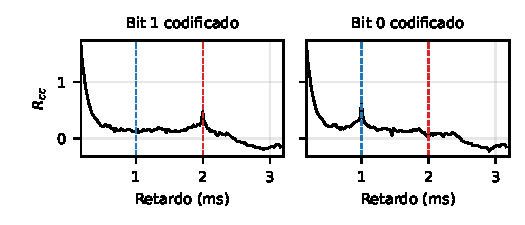
\includegraphics[width=\columnwidth]{rcc.pdf}
\caption{$R_{cc}$ promedio de 20 ventanas con un 1 (izquierda) y un 0 (derecha) codificados; las líneas marcan $t_1$ y $t_0$.}
\label{fig:rcc}
\end{figure}

\subsection{Amplitud del eco y calidad}
La Figura~\ref{fig:vsa} presenta recuperación y PESQ frente a $a$. Con $a=0.1$ la recuperación es $\approx$81\% en las tres pistas y con $a=0.5$ supera 98\%; en cambio, el PESQ promedio cae de 4.3 a 2.7. Esto concuerda con la teoría: el pico de $R_{cc}$ crece con $a$, pero el eco se vuelve audible. Con $a=0.3$ la recuperación es 98.8\%, 97.7\% y 96.5\% (clásica, folk y jazz), cumpliendo el 90\% exigido; el PESQ es 4.00, 3.61 y 2.67. El jazz es el más afectado, pues su contenido denso en armónicos produce más estructura cepstral propia.

\begin{figure}[t]
\centering
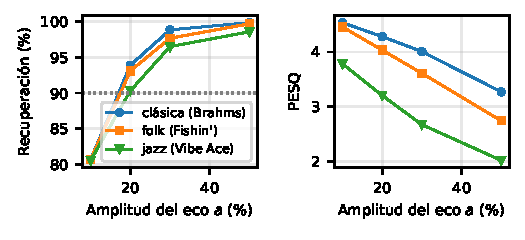
\includegraphics[width=\columnwidth]{vs_a.pdf}
\caption{Tasa de recuperación (izquierda) y PESQ (derecha) frente a la amplitud del eco, con $L=8t_{max}$.}
\label{fig:vsa}
\end{figure}

\subsection{Longitud de ventana y retardos}
La Tabla~\ref{tab:ventana} muestra el compromiso entre tasa de transferencia y recuperación con $a=0.3$: ventanas más largas incluyen más ciclos del eco, aumentan la recuperación y el PESQ, pero reducen la tasa. Con $L=t_{max}$ el sistema no es útil (56\%).

\begin{table}[t]
\centering
\caption{Efecto de la longitud de ventana ($a=0.3$; promedio de las tres pistas)}
\label{tab:ventana}
\begin{tabular}{rrrrr}
\toprule
$L/t_{max}$ & $L$ (muestras) & Tasa (b/s) & Recuperación (\%) & PESQ \\
\midrule
1 & 88 & 501.1 & 55.7 & 2.36 \\
2 & 176 & 250.6 & 82.2 & 2.63 \\
4 & 352 & 125.3 & 93.4 & 2.99 \\
8 & 704 & 62.6 & 97.7 & 3.43 \\
16 & 1408 & 31.3 & 98.9 & 3.70 \\
\bottomrule
\end{tabular}
\end{table}

Para los retardos (con $L=8t_{max}$), la recuperación promedio fue 94.7\% con 0.5 y 1~ms; 97.7\% con 1 y 1.5~ms; 97.3\% con 1 y 2~ms; 97.9\% con 2 y 3~ms; y 99.0\% con 2 y 4~ms. Retardos largos facilitan la separación de los picos y alargan la ventana (menor tasa), como describe la teoría. El PESQ no es monótono (3.17, 3.37, 3.44, 3.55 y 3.07), porque la audibilidad depende también del tipo de retardo (eco fusionado con la señal frente a eco separado).

\subsection{Calidad, recuperación y tasa de transferencia}
La Figura~\ref{fig:corr} grafica el PESQ frente a la recuperación para las 48 configuraciones de la barrida (amplitud y ventana). La correlación de Spearman entre recuperación y PESQ es $\rho=-0.25$, y entre tasa de transferencia y PESQ, $\rho=-0.31$. Ambas son débiles y negativas: lo que aumenta la recuperación (más amplitud) degrada el PESQ, mientras que el efecto de la ventana es el contrario, y la mezcla de ambos factores oculta la tendencia. La tasa de transferencia y la recuperación sí se oponen con claridad ($\rho=-0.61$).

\begin{figure}[t]
\centering
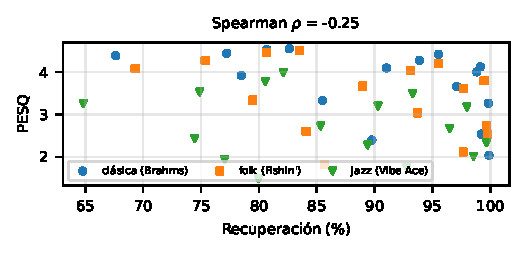
\includegraphics[width=\columnwidth]{pesq_rec.pdf}
\caption{PESQ frente a la tasa de recuperación para las configuraciones evaluadas.}
\label{fig:corr}
\end{figure}

\subsection{Ruido, ventanas sin eco y mensaje completo}
Como análisis propio, se añadió ruido blanco gaussiano (Figura~\ref{fig:ruido}). La recuperación por ventana baja de 97.7\% (sin ruido) a $\approx$83\% con 20~dB de relación señal a ruido (SNR). Aun así, la suma de copias recupera el mensaje completo en la pista folk hasta 20~dB y en la clásica hasta 30~dB; en jazz solo sin ruido. La detección de ventanas sin eco (umbral $\theta=2$) falla en 5.5--13.7\% de las ventanas codificadas y marca como codificadas 7.9--18.4\% de las no codificadas. Como las ventanas dudosas no votan, esto no afecta al mensaje. Con tres metadatos, el mensaje se recuperó en las tres pistas desde 30~s de audio (con 15~s solo en la clásica), pues con menos duración hay pocas copias que sumar.

\begin{figure}[t]
\centering
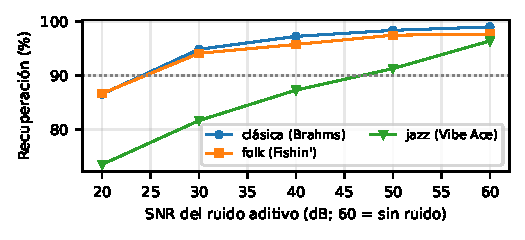
\includegraphics[width=\columnwidth]{ruido.pdf}
\caption{Tasa de recuperación por ventana frente a la SNR del ruido aditivo.}
\label{fig:ruido}
\end{figure}

\subsection{Limitaciones}
Solo se probaron tres pistas, una por género; el PESQ no es una medida de calidad musical y no se hicieron pruebas auditivas. Los errores por ventana dependen de la señal y llegan en ráfagas; por eso repetir bits adyacentes no mejoró la recuperación del mensaje, y fue necesario repetir el mensaje completo en el archivo.

\section{Conclusiones}
\begin{enumerate}
\item Los picos de $R_{cc}$ aparecen en el retardo codificado y permiten decidir el bit; promediar con y sin ventana de Hann mejora la decisión en señales tonales.
\item Con $a=0.3$, la recuperación por ventana es 96.5--98.8\% y cumple el requisito de 90\%; subir $a$ la aumenta a costa del PESQ.
\item La ventana $L=t_{max}$ solo alcanza 56\% de recuperación; $L=8t_{max}$ alcanza 97.7\% con 62.6~b/s, y duplicarla ofrece solo 1.2 puntos más al costo de la mitad de la tasa.
\item Los retardos largos mejoran la recuperación y disminuyen la tasa, sin efecto monótono sobre el PESQ.
\item La correlación entre recuperación, tasa y PESQ es débil, salvo el compromiso entre tasa y recuperación ($\rho=-0.61$).
\item La suma de copias del mensaje, con Hamming y CRC, permite recuperar los metadatos desde 30~s de audio y tolerar ruido de 20 a 30~dB según el género.
\end{enumerate}
Como trabajo futuro se recomienda: probar más canciones y pruebas de escucha; adaptar $a$ a la ventana según su energía; incorporar resistencia a la compresión con pérdida; y explorar la ejecución en línea con altavoz y micrófono.

\begin{thebibliography}{1}
\bibitem{kim} P.~Dutta, D.~Bhattacharyya y T.~Kim, ``Data hiding in audio signal: a review,'' \textit{Int. J. Database Theory and Application}, vol.~2, 2009.
\bibitem{behal} S.~Behal y N.~Kaur, ``Audio steganography techniques - a survey,'' \textit{Int. J. Engineering Research and Applications}, vol.~4, pp.~94--100, 2014.
\bibitem{gruhl} D.~Gruhl, A.~Lu y W.~Bender, ``Echo hiding,'' Informe técnico, MIT Media Laboratory.
\bibitem{korzhik} V.~Korzhik, ``Audio watermarking based on echo hiding with zero error probability,'' \textit{Int. J. Computer Science and Applications}, vol.~10, pp.~1--10, 2013.
\bibitem{pesq} ITU-T, ``P.862: Perceptual evaluation of speech quality (PESQ),'' 2018.
\end{thebibliography}
\end{document}
